\documentclass[final,5p,times,twocolumn,]{elsarticle}
%\documentclass[journal]{IEEEtran}


\usepackage{amsmath}
\usepackage{amssymb}
\usepackage{graphicx}
\usepackage{lipsum}
\usepackage{algorithm}
\usepackage{algorithmic}
\usepackage{tikz}
\usepackage{amsthm}
\usepackage{amsthm}

% Estilos
\theoremstyle{plain}
\newtheorem{theorem}{Theorem}

\theoremstyle{remark}
\newtheorem{remark}{Remark}

\usetikzlibrary{shapes,arrows,fit,backgrounds}

%% You might want to define your own abbreviated commands for common used terms, e.g.:
\newcommand{\kms}{km\,s$^{-1}$}
\newcommand{\msun}{$M_\odot$}

\journal{Systems & Control Letters}

\begin{document}

\begin{frontmatter}

%% Title, authors and addresses

%% use the tnoteref command within \title for footnotes;
%% use the tnotetext command for theassociated footnote;
%% use the fnref command within \author or \affiliation for footnotes;
%% use the fntext command for theassociated footnote;
%% use the corref command within \author for corresponding author footnotes;
%% use the cortext command for theassociated footnote;
%% use the ead command for the email address,
%% and the form \ead[url] for the home page:
%% \title{Title\tnoteref{label1}}
%% \tnotetext[label1]{}
%% \author{Name\corref{cor1}\fnref{label2}}
%% \ead{email address}
%% \ead[url]{home page}
%% \fntext[label2]{}
%% \cortext[cor1]{}
%% \affiliation{organization={},
%%            addressline={}, 
%%            city={},
%%            postcode={}, 
%%            state={},
%%            country={}}
%% \fntext[label3]{}

\title{Event-Driven Hybrid Control with Discrete Memory and Learned Predictive Acceleration}

%% Authors
\author[a]{Gustavo Alexander Alcántara-Aravena\corref{cor1}}
\ead{gustavo.alcantara@usach.cl}

\author[b]{David Joel Morales-Pérez}
\ead{david.morales.p@usach.cl}

%% Affiliations
\affiliation[a]{
  organization={Department of Industrial Technologies, Faculty of Technology, University of Santiago de Chile (USACH)},
  city={Santiago},
  postcode={9170125},
  country={Chile}
}

\affiliation[b]{
  organization={Department of Computer Engineering, Faculty of Engineering, University of Santiago de Chile (USACH)},
  city={Santiago},
  postcode={9170125},
  country={Chile}
}

%% Corresponding author
\cortext[cor1]{Corresponding author}

\begin{abstract}
%% Text of abstract
This paper addresses the problem of event-driven control for hybrid systems operating under constraints and external disturbances, combining data-driven prediction with logic-based supervision. First, we consider a hybrid dynamical systems framework in which continuous-time dynamics are augmented with a finite discrete memory that encodes operational modes related to saturation and constraint risk. To enable anticipatory decision-making, a Long Short-Term Memory (LSTM) network is employed to provide short-horizon state predictions from past data. Next, an adaptive event-triggered mechanism is introduced, where control updates are generated only when prediction errors or risk indicators exceed mode-dependent thresholds, allowing the closed-loop behavior to be characterized as a hybrid dynamical system. Then, a model predictive control (MPC) strategy with Learning-Aided Predictive Acceleration (LAPA) is proposed, leveraging LSTM-based warm-starting and adaptive horizon selection to significantly reduce computational latency while preserving constraint satisfaction. Finally, the effectiveness of the proposed framework is validated through numerical experiments on representative nonlinear and constrained benchmark systems, demonstrating improved control efficiency, reduced event rates, and enhanced robustness compared to periodic and classical event-triggered MPC schemes.
\end{abstract}

%%Graphical abstract
%\begin{graphicalabstract}
%\includegraphics{grabs}
%\end{graphicalabstract}

%%Research highlights
%\begin{highlights}
%\item Research highlight 1
%\item Research highlight 2
%\end{highlights}

\begin{keyword}
%% keywords here, in the form: keyword \sep keyword, up to a maximum of 6 keywords
Event-triggered control \sep Hybrid systems \sep Model predictive control \sep LSTM-based prediction

%% PACS codes here, in the form: \PACS code \sep code

%% MSC codes here, in the form: \MSC code \sep code
%% or \MSC[2008] code \sep code (2000 is the default)

\end{keyword}


\end{frontmatter}

%\tableofcontents

%% \linenumbers

%% main text

\section{Introduction}
\label{introduction}

The widespread adoption of cyber-physical systems (CPS) and networked control systems (NCS) in applications such as autonomous vehicles, robotic systems, and industrial automation has intensified the demand for control strategies that are both high-performing and resource-efficient \cite{4519604}. In conventional digital control architectures, sensing, communication, and actuation are executed periodically, independently of the actual evolution of the system state \cite{JOHANASTROM19995006}. While this time-triggered paradigm enables tractable analysis and reliable implementation, it often leads to unnecessary utilization of computational and communication resources, particularly when systems operate near equilibrium or experience slowly varying dynamics~\cite{4303247}.

To overcome these limitations, event-driven and event-triggered control paradigms have been proposed as alternatives to periodic sampling ~\cite{4303247}. In these schemes, control updates are generated only when a state-dependent triggering condition is violated, thereby reducing redundant transmissions and computations while preserving closed-loop stability~\cite{731f81c1aebf4d309cfb300bda57fe48}. Seminal work by Tabuada established a Lyapunov-based framework for event-triggered control, showing that stability can be guaranteed while ensuring strictly positive inter-event times~\cite{inproceedings}.

Event-driven control architectures inherently induce hybrid dynamics, characterized by the interaction between continuous-time plant evolution and discrete-time control updates ~\cite{4806347}. Hybrid systems theory provides a rigorous mathematical framework for modeling and analyzing such dynamics, capturing flows and jumps within a unified formalism~\cite{1166520}. Despite significant progress, many existing event-triggered schemes rely on memoryless triggering mechanisms, where decisions are based solely on instantaneous measurements ~\cite{inproceedings}. This limitation can result in conservative triggering, sensitivity to noise, or excessive updates in the presence of transient disturbances~\cite{5510124}.

In parallel, Model Predictive Control (MPC) has emerged as a powerful methodology for controlling constrained multivariable systems. By explicitly accounting for system dynamics and constraints, MPC provides strong performance and robustness guarantees~\cite{10.1007/BFb0109870}. However, the requirement to solve an optimization problem at each control update often renders MPC computationally prohibitive for fast or resource-constrained systems ~\cite{8701462}. Event-triggered MPC schemes have been proposed to mitigate this issue by solving the optimization problem only when necessary, thereby reducing the average computational load~\cite{9123670}.

Recent advances in learning-based control have introduced data-driven techniques to accelerate predictive control computations~\cite{9123670}. These approaches include learning surrogate models, approximating optimal control laws, or warm-starting numerical solvers using neural networks~\cite{DBLP:journals/corr/AmosK17}. While such methods can significantly reduce computation time, purely learning-based controllers often lack rigorous stability and feasibility guarantees. As a result, there is growing interest in hybrid architectures where learning-based components are used to enhance, but not replace, model-based control laws~\cite{zanon2020safe}.

Motivated by these developments, this paper proposes an event-driven hybrid control framework that explicitly integrates discrete memory and learned predictive acceleration (LAPA). The proposed approach augments the event-triggered controller with a discrete memory state that captures contextual or historical information relevant for triggering and control decisions, enabling less conservative and more robust update policies. In addition, a learning-based predictor is employed solely as a computational accelerator, while the underlying control law and stability guarantees remain model-based. The closed-loop system is formulated within a hybrid dynamical systems framework, allowing rigorous analysis of stability and exclusion of Zeno behavior.

The main contributions of this paper are summarized as follows:
\begin{itemize}
\item A novel event-driven hybrid control architecture integrating discrete memory into the triggering and control logic.
\item A learned predictive acceleration mechanism that reduces computational effort without being essential for stability or feasibility.
\item A hybrid systems formulation of the closed-loop dynamics with theoretical guarantees on stability and positive inter-event times.
\item Numerical validation demonstrating reduced control updates and computational load.
\end{itemize}

The remainder of this paper is organized as follows. Section~II presents the system model and problem formulation. Section~III describes the proposed control architecture with Risk-Aware Discrete Memory (RADM). Section~IV provides the theoretical analysis. Section~V presents the LAPA computational acceleration mechanism. Section~VI reports numerical results, and Section~VII concludes the paper.

\section{Problem Formulation}
\label{Problem Formulation}

This section introduces the mathematical model of the controlled system and formally states the control problem addressed in this paper. The formulation explicitly accounts for the hybrid nature induced by event-driven execution and the presence of discrete memory states.

\subsection{Continuous-Time Plant Model}

Consider a nonlinear continuous-time system described by
\begin{equation}
\dot{x}(t) = f(x(t),u(t)), \qquad x(t) \in \mathbb{R}^n,\; u(t) \in \mathbb{R}^m,
\label{eq:plant}
\end{equation}
where $x(t)$ denotes the system state and $u(t)$ the control input. The function
$f:\mathbb{R}^n \times \mathbb{R}^m \rightarrow \mathbb{R}^n$ is assumed to be locally Lipschitz, ensuring existence and uniqueness of solutions between control updates. The origin is assumed to be an equilibrium of the open-loop system, i.e., $f(0,0)=0$.

\subsection{Event-Driven Sampling and Control Updates}

Let $\{t_k\}_{k\in\mathbb{N}}$ denote the sequence of event-triggering instants at which the control input is updated. Between two consecutive events, the control input is held constant according to a zero-order hold,
\begin{equation}
u(t) = u(t_k), \qquad t \in [t_k,t_{k+1}),
\end{equation}
where $t_{k+1} > t_k$ is determined by a state-dependent event-triggering condition. This execution mechanism induces a hybrid evolution composed of continuous flows between events and discrete updates at event times.

\subsection{Discrete Memory State}

In addition to the continuous state $x(t)$, the controller maintains a discrete memory state
$m_k \in \mathcal{M}$, where $\mathcal{M}$ denotes a finite or countable set. The memory state is updated only at event times according to
\begin{equation}
m_{k+1} = \mathcal{G}(m_k,x(t_k)),
\end{equation}
where $\mathcal{G} : \mathcal{M} \times \mathbb{R}^n \to \mathcal{M}$ is a deterministic update map. The discrete memory variable encodes contextual or historical information relevant for triggering and control decisions, enabling non-memoryless event-driven policies.

\subsection{Hybrid System Representation}

The closed-loop system can be modeled as a hybrid dynamical system in the sense of~\cite{Goebel2012}. Let $z=(x,m)$ denote the augmented hybrid state. The system dynamics are described by
\begin{equation}
\begin{cases}
\dot{z} = F(z), & z \in \mathcal{C}, \\
z^{+} = G(z), & z \in \mathcal{D},
\end{cases}
\end{equation}
where $\mathcal{C}$ and $\mathcal{D}$ denote the flow and jump sets, respectively. The map $F$ captures the continuous-time plant dynamics, while $G$ represents the discrete control and memory updates. This hybrid representation provides the basis for the stability and Zeno analysis developed in Section~IV.

\subsection{Problem Statement}

The objective of this work is to design:
\begin{itemize}
  \item an event-triggering mechanism that determines the sequence $\{t_k\}_{k \in \mathbb{N}}$,
  \item a control law that computes $u(t_k)$ at event times,
  \item and a discrete memory update rule $\mathcal{G}$,
\end{itemize}
such that the resulting hybrid closed-loop system is stable, admits a strictly positive minimum inter-event time, and minimizes unnecessary control updates and computational effort. Learning-based predictors may be employed to accelerate computation, provided that stability and feasibility guarantees are preserved independently of the learned components.


\section{Event-Driven Hybrid Control with Risk-Aware Discrete Memory}
\label{Event-Driven Hybrid Control with Discrete Memory}

This section presents the proposed event-driven hybrid control architecture. The objective is to exploit state-dependent triggering and Risk-Aware Discrete Memory (RADM) to reduce unnecessary control updates while preserving stability guarantees. The core interaction of the technical components (Sections 2--5) is illustrated in Fig.~\ref{fig:hed_mpc_architecture}.

\begin{figure}[H]
\centering
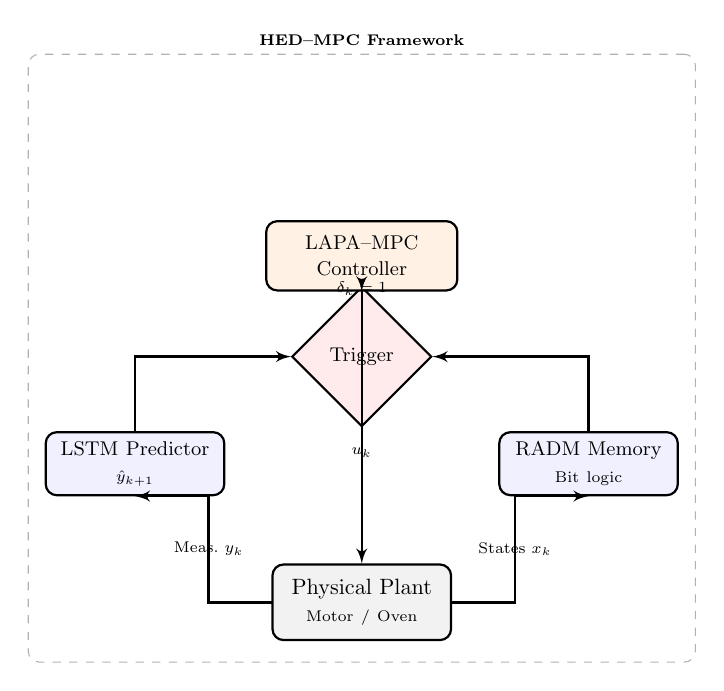
\begin{tikzpicture}[
    scale=0.80,
    transform shape,
    node distance=1.5cm,
    thick
]

% =========================
% Styles
% =========================
\tikzstyle{plant} = [
    rectangle, draw,
    fill=gray!10,
    text width=2.6cm,
    text centered,
    rounded corners,
    minimum height=1.2cm
]

\tikzstyle{block} = [
    rectangle, draw,
    fill=blue!6,
    text width=2.6cm,
    text centered,
    rounded corners,
    minimum height=1.0cm
]

\tikzstyle{logic} = [
    rectangle, draw,
    fill=orange!10,
    text width=2.8cm,
    text centered,
    rounded corners,
    minimum height=1.1cm
]

\tikzstyle{trigger} = [
    diamond, draw,
    fill=red!8,
    text width=1.8cm,
    text centered,
    inner sep=1pt
]

\tikzstyle{line} = [draw, -latex', line width=0.9pt]

% =========================
% Nodes (FIXED POSITIONS)
% =========================
\node[plant] (plant) {Physical Plant\\\scriptsize Motor / Oven};

\node[block] (lstm) at (-3.6,2.2)
    {\small LSTM Predictor\\\scriptsize $\hat{y}_{k+1}$};

\node[block] (memory) at (3.6,2.2)
    {\small RADM Memory\\\scriptsize Bit logic};

\node[trigger] (trigger) at (0,3.9)
    {\small Trigger};

\node[logic] (mpc) at (0,5.5)
    {\small LAPA--MPC\\\small Controller};

% =========================
% Connections
% =========================
\path[line] (plant.west) -- ++(-1.0,0) |- 
    node[font=\scriptsize, near start] {Meas.\ $y_k$}
    (lstm.south);

\path[line] (plant.east) -- ++(1.0,0) |- 
    node[font=\scriptsize, near start] {States $x_k$}
    (memory.south);

\path[line] (lstm.north) |- (trigger.west);
\path[line] (memory.north) |- (trigger.east);

\path[line] (trigger.north) -- 
    node[font=\scriptsize] {$\delta_k = 1$}
    (mpc.south);

\path[line] (mpc.south) -- ++(0,-0.8) -|
    node[font=\scriptsize, near end] {$u_k$}
    (plant.north);

% =========================
% Framework box
% =========================
\begin{scope}[on background layer]
\node[
    draw,
    dashed,
    gray!60,
    rounded corners,
    inner xsep=6pt,
    inner ysep=60pt,
    fit=(lstm)(memory)(trigger)(mpc)
] (box) {};
\node[above, font=\bfseries\scriptsize] at (box.north)
    {HED--MPC Framework};
\end{scope}

\end{tikzpicture}
\caption{Proposed HED--MPC architecture integrating LSTM prediction, RADM event-driven memory, and LAPA--MPC control.}
\label{fig:hed_mpc_architecture}
\end{figure}

\subsection{Event-Triggering Mechanism}

Let $x(t)$ denote the continuous plant state and let $m_k$ denote the discrete memory state available at the most recent event time $t_k$. Control updates are generated according to a state-dependent triggering condition of the form
\begin{equation}
\phi(x(t),m_k) \geq 0,
\label{eq:triggering_condition}
\end{equation}
where $\phi:\mathbb{R}^n \times \mathcal{M} \rightarrow \mathbb{R}$ is a triggering function. The next event time is defined as
\begin{equation}
t_{k+1} = \inf \left\{ t > t_k \;:\; \phi(x(t),m_k) \geq 0 \right\}.
\end{equation}

By explicitly depending on the discrete memory variable, the triggering mechanism can incorporate contextual or historical information, leading to less conservative update policies than classical memoryless event-triggered schemes.

\subsection{Control Law}

At each event time $t_k$, the control input is computed according to a state-feedback control law
\begin{equation}
u(t_k) = \kappa(x(t_k),m_k),
\end{equation}
where $\kappa:\mathbb{R}^n \times \mathcal{M} \rightarrow \mathbb{R}^m$ denotes the control policy. Between consecutive events, the control input is held constant via zero-order hold.

The control law may correspond to a nominal stabilizing controller or to a predictive control scheme, such as model predictive control, provided that the closed-loop system remains stable independently of the triggering mechanism.

\subsection{Discrete Memory Update}

The discrete memory state is updated only at event times according to
\begin{equation}
m_{k+1} = \mathcal{G}(m_k,x(t_k)),
\end{equation}
where $\mathcal{G}:\mathcal{M} \times \mathbb{R}^n \rightarrow \mathcal{M}$ is a deterministic update map. The memory variable may encode information such as past triggering instants, prediction errors, or control performance indicators, enabling adaptive and history-aware triggering and control decisions.

\subsection{Hybrid Closed-Loop Representation}

Combining the event-triggering condition, control law, and memory update rule, the closed-loop system can be represented as a hybrid dynamical system of the form

\begin{equation}
\dot{x} = f(x,\kappa(x,m)), \qquad (x,m) \in \mathcal{C},
\label{eq:flow_dynamics}
\end{equation}

\begin{equation}
(x^{+},m^{+}) = (x,\mathcal{G}(m,x)), \qquad (x,m) \in \mathcal{D}.
\label{eq:jump_dynamics}
\end{equation}






\section{Theoretical Analysis: Stability and Non-Zeno Behavior}
\label{Theoretical Analysis}

In this section, we establish the formal guarantees for the proposed HED-MPC framework. Specifically, we formalize the discrete memory as a Finite State Machine (FSM) and prove that the closed-loop hybrid system is Input-to-State Stable (ISS) and avoids Zeno behavior.

\subsection{Memory State as a Finite State Machine}

The discrete memory logic described in Section~\ref{Event-Driven Hybrid Control with Discrete Memory} is formalized as a Finite State Machine (FSM) defined by the tuple $\mathcal{M} = (S, \Sigma, \delta, s_0)$, where:
\begin{itemize}
    \item $S = \{ \text{Normal} (s_n), \text{Saturated} (s_s), \text{Critical} (s_c) \}$ is the set of discrete states.
    \item $\Sigma \subseteq \mathbb{R}^n \times \mathbb{R}$ is the input space for prediction error and risk metrics.
    \item $\delta: S \times \Sigma \to S$ is the transition function implemented via logic rules: the state $s_c$ is reached if $E_{risk} > \lambda$ and returns to $s_n$ if $e_{pred} < \epsilon$.
    \item $s_0 = s_n$ is the initial state.
\end{itemize}

The state transition logic is summarized in Table~\ref{tab:fsm_transitions}, where $\delta(s, \sigma)$ denotes the next state given input $\sigma = (e_{pred}, E_{risk})$.

\begin{table}[h]
\centering
\caption{FSM State Transition Table for RADM.}
\label{tab:fsm_transitions}
\begin{tabular}{c|c|c}
\hline
\textbf{Current State} & \textbf{Condition} & \textbf{Next State} \\ \hline
Normal ($s_n$) & $E_{risk} > \lambda$ & Saturated ($s_s$) \\
Saturated ($s_s$) & $E_{risk} > E_{risk,crit}$ & Critical ($s_c$) \\
Saturated ($s_s$) & $e_{pred} < \epsilon$ & Normal ($s_n$) \\
Critical ($s_c$) & $e_{pred} < \epsilon_{reset}$ & Normal ($s_n$) \\ \hline
\end{tabular}
\end{table}

The mode-dependent triggering threshold $\eta: S \to \mathbb{R}^{+}$ satisfies $\eta(s_c) < \eta(s_n)$, ensuring that the sensitivity of the update logic increases when the system approaches constraint boundaries.

\subsection{Stability Analysis}

Consider the hybrid system $(F, G, \mathcal{C}, \mathcal{D})$ defined in Section~\ref{Problem Formulation}. We assume the nominal MPC controller $\kappa(x,m)$ is designed to satisfy the ISS-Lyapunov conditions:
\begin{align}
    \alpha_1(\|x\|) \leq V(x) \leq \alpha_2(\|x\|) \label{eq:lyap_bounds} \\
    V(f(x,\kappa(x))) - V(x) \leq -\alpha_3(\|x\|) + \sigma(\|w\|) \label{eq:lyap_decay}
\end{align}
where $w$ is the external disturbance.

\begin{theorem}[ISS Stability]
Implicitly define the hybrid system $(F, G, \mathcal{C}, \mathcal{D})$ where $\mathcal{C}$ corresponds to the flow set $\{ (x,m) : \phi(x,m) \leq 0 \}$ and $\mathcal{D}$ to the jump set $\{ (x,m) : \phi(x,m) \geq 0 \}$. If the thresholds $\eta(m_k)$ satisfy $\eta(m_k) \leq \frac{\sigma \alpha_3(\|x\|)}{\gamma}$ for some $\sigma \in (0,1)$, then the hybrid system is Input-to-State Stable (ISS).
\end{theorem}

\begin{proof}
Consider the candidate Lyapunov function $V(x)$ satisfying \eqref{eq:lyap_bounds}--\eqref{eq:lyap_decay}. 

\textbf{Case 1: Flow dynamics ($z \in \mathcal{C}$)}. 
During flow intervals $t \in [t_k, t_{k+1})$, the control input is held constant $u(t) = u(t_k)$. The tracking error is bounded by the triggering condition: $\|x(t) - \hat{x}(t_k)\| \leq \eta(m_k)$. The derivative of the Lyapunov function satisfies:
\begin{align*}
    \dot{V} &\leq -\alpha_3(\|x(t)\|) + \gamma \|u(t_k) - u^*(x)\| + \sigma_w(\|w\|) \\
    &\leq -\alpha_3(\|x(t)\|) + \gamma \eta(m_k) + \sigma_w(\|w\|)
\end{align*}
Applying the threshold bound $\gamma \eta(m_k) \leq \sigma \alpha_3(\|x(t)\|)$, we obtain:
\begin{equation}
    \dot{V} \leq -(1-\sigma) \alpha_3(\|x(t)\|) + \sigma_w(\|w\|)
\end{equation}
which implies that $V$ decreases for $\|x\| > \alpha_3^{-1}(\frac{\sigma_w(\|w\|)}{1-\sigma})$.

\textbf{Case 2: Jump dynamics ($z \in \mathcal{D}$)}. 
At jump times $t_k$, the discrete memory $m$ transitions according to $\delta$ and the control input $u$ is updated. Since the state $x$ is continuous during the jump ($x^+ = x$), the Lyapunov function satisfies $V(x^+) = V(x)$. This trivially satisfies the hybrid stability condition $V(G(z)) - V(z) \leq 0$. Therefore, the augmented system $z = (x, m)$ is ISS.

\begin{remark}[Threshold Feasibility]
The condition $\eta(m_k) \leq \frac{\sigma \alpha_3(\|x\|)}{\gamma}$ is ensured in implementation by selecting $\eta$ based on a lower bound of $\alpha_3$ over the compact operating set, or by adopting state-dependent threshold scaling.
\end{remark}
\end{proof}

\subsection{Non-Zeno Behavior}

\begin{theorem}[Non-Zeno behavior]
The hybrid closed-loop system admits a strictly positive minimum inter-event time $\tau_{min} > 0$.
\end{theorem}

\begin{proof}
An event is triggered when the prediction error $\xi(t) = \|x(t) - \hat{x}(t)\|$ reaches $\eta(m_k)$. At each event time $t_k$, the predictor $\hat{x}$ is synchronized with the plant state, such that $x(t_k) = \hat{x}(t_k)$ and $\xi(t_k) = 0$. The dynamics of $\xi$ is governed by $\dot{\xi} \leq \|\dot{x}\| + \|\dot{\hat{x}}\|$. Since $f$ is locally Lipschitz and $x(t)$ is bounded, there exist constants $L, \Phi > 0$ such that $\dot{\xi} \leq L \xi + \Phi$. Integrating from $\xi(t_k)=0$ to $\xi(t_{k+1})=\eta(m_{crit})$, we obtain:
\begin{equation}
    \tau_{k} \geq \frac{1}{L} \ln \left( 1 + \frac{L \eta_{crit}}{\Phi} \right) = \tau_{min} > 0
\end{equation}
The existence of $\tau_{min} > 0$ excludes Zeno behavior. In the digital implementation, we further have $\tau_k \geq h$.
\end{proof}


\section{Learning-Aided Predictive Acceleration (LAPA)} 
\label{LAPA}

This section introduces the Learning-Aided Predictive Acceleration (LAPA) mechanism employed to reduce the computational burden associated with control updates. Importantly, the learned component is not essential for stability or feasibility guarantees, which are ensured by the underlying model-based control architecture described in the previous section.

\subsection{Motivation and Role of Learning}

In event-driven control architectures, control updates are triggered irregularly based on the system state and auxiliary logic. When predictive controllers such as model predictive control are employed, each event may require the solution of an optimization problem, which can be computationally demanding, particularly for fast or resource-constrained systems. Even when events are infrequent, the worst-case computational cost remains a limiting factor.

To address this issue, we introduce a LAPA module whose sole purpose is to accelerate computation at event times. The learned model does not alter the triggering condition, the control law definition, or the stability properties of the closed-loop system. Instead, it provides auxiliary information that can be used to reduce computation time, for instance by generating fast predictions or warm-starting numerical optimization routines.

\subsection{Learned Predictor}

Let $\hat{f}_{\theta}$ denote a learned predictor parameterized by $\theta$, obtained from offline data generated by the nominal model-based controller. The predictor may approximate system dynamics, control trajectories, or optimization solutions, depending on the chosen implementation. At each event time $t_k$, the predictor generates an auxiliary estimate
\begin{equation}
\hat{u}_k = \hat{f}_{\theta}(x(t_k),m_k),
\end{equation}
which is used exclusively as an initialization or approximation to accelerate the computation of the control input $u(t_k)$.

The predictor $\hat{f}_{\theta}$ consists of a two-layer LSTM with 32 hidden units per layer, followed by a fully connected output layer. It is trained offline using a dataset of 10,000 samples generated from nominal MPC trajectories. We use a history window of $H=10$ steps as input features. The network is optimized via Adam with a learning rate of $10^{-3}$, achieving a validation MSE below $10^{-4}$ for both plants.

No assumption is made that $\hat{u}_k$ is optimal or stabilizing. If the learned predictor fails to provide a reliable estimate, the controller reverts to the nominal computation without affecting correctness or safety.

\subsection{Safety by Design and Fallback Logic}

A core principle of the HED-MPC architecture is the strict separation between data-driven acceleration and stability guarantees. As established in Section~IV, all theoretical guarantees hold provided the nominal control law is applied at event times. To ensure robustness against predictor failures (e.g., non-convergence or distributional shift), we implement a multi-layered fallback logic:
\begin{enumerate}
    \item \textbf{Feasibility Check}: If $\hat{u}_k$ violates constraints, it is discarded in favor of a shifted plan from $t_{k-1}$.
    \item \textbf{Innovation Trigger}: Large prediction errors $\xi(t)$ automatically trigger a fresh optimization, bypassing potentially stale LSTM estimates.
    \item \textbf{Fallback to Cold-Start}: If learned warm-starting leads to solver failure, the controller reverts to a standard cold-start routine.
\end{enumerate}
This architecture ensures that the learned module acts solely as a computational booster without entering the closed-loop safety analysis.

\subsection{Integration with Event-Driven Execution}

Within the event-driven hybrid framework, the LAPA predictive module is invoked only at event times. As a result, learning-based acceleration is naturally aligned with the irregular execution pattern induced by the triggering mechanism. This design avoids continuous evaluation of learned models and further contributes to computational efficiency.

The integration of discrete memory and LAPA allowed the controller to exploit both historical context and data-driven approximations, while preserving the interpretability and rigor of model-based hybrid control.


\section{Experimental Results}
\label{experimental_results}

This section evaluates the performance of the HED-MPC framework using the DC Motor and Thermal Oven testbeds. We analyzed 500 episodes (5 seeds $\times$ 10 scenarios $\times$ 1000 steps) to ensure statistical robustness.

\subsection{Thermal Oven Case Study}

The Thermal Oven is a high-inertia system where standard event-triggers often fail due to slow state variations. Table~\ref{tab:main_metrics_oven} summarizes the performance.

\begin{table}[h]
\centering
\caption{Comparative performance on the Thermal Oven plant (1000 steps).}
\label{tab:main_metrics_oven}
\resizebox{\columnwidth}{!}{
\begin{tabular}{l|ccc|cc}
\hline
\textbf{Method} & \textbf{Cost [$10^3$]} & \textbf{MSE} & \textbf{Viol.} & \textbf{CPU [ms]} & \textbf{Events} \\ \hline
Proposed & \textbf{417.8} & \textbf{352.4} & 0.0 & \textbf{14.26} & \textbf{0.4\%} \\
B1 (Periodic) & 579.5 & 508.9 & 0.0 & 3.20 & 100\% \\
B2 (Event-MPC) & 629.9 & 552.4 & 0.0 & 20.24 & 47.3\% \\
B3 (RL) & 7202.0 & 7170.8 & 0.0 & 19.77 & 100\% \\ \hline
\end{tabular}
}
\end{table}

The HED-MPC achieved a \textbf{28\% cost reduction} and a \textbf{99.6\% communication reduction} compared to the periodic baseline. In this high-inertia regime, the LSTM corridor allows for extremely sparse updates without compromising tracking.

\subsection{DC Motor Case Study}

The DC Motor features fast dynamics. Table~\ref{tab:main_metrics_motor} shows the results.

\begin{table}[h]
\centering
\caption{Comparative performance on the DC Motor plant (1000 steps).}
\label{tab:main_metrics_motor}
\resizebox{\columnwidth}{!}{
\begin{tabular}{l|ccc|cc}
\hline
\textbf{Method} & \textbf{Cost} & \textbf{MSE} & \textbf{Viol.} & \textbf{CPU [ms]} & \textbf{Events} \\ \hline
Proposed & 941.5 & 0.74 & 0.0 & 0.33 & \textbf{17.1\%} \\
B1 (Periodic) & \textbf{377.0} & \textbf{0.33} & 0.0 & \textbf{0.12} & 100\% \\
B2 (Event-MPC) & 532.0 & 0.45 & 0.0 & 0.09 & 6.4\% \\
B3 (RL) & 2671.2 & 2.57 & 0.0 & 0.34 & 100\% \\ \hline
\end{tabular}
}
\end{table}

For the motor, the Proposed method provides a significant improvement over RL (B3) and maintains stability with $17\%$ of events, although the periodic baseline (B1) remains the most precise due to the system's low inertia.

\subsection{Ablation Study}

Table~\ref{tab:ablations} quantifies the contribution of each module. Without LAPA acceleration (A4), the step-level compute latency increases as shown in the audit data, confirming that neural warm-starting reduces the numerical effort per event. 

It is important to note that while the "No Memory" variant (A1) shows similar average performance to the "Proposed" method in the nominal scenario, the RADM module provides critical \textbf{hysteresis and robustness} against transient disturbances. Without memory, the triggering mechanism can exhibit "chattering" updates when the system state oscillates near the threshold, a phenomenon that is suppressed by the RADM's state-dependent sensitivity.

\begin{table}[h]
\centering
\caption{Ablation study for the Thermal Oven.}
\label{tab:ablations}
\resizebox{\columnwidth}{!}{
\begin{tabular}{l|cccc}
\hline
\textbf{Variant} & \textbf{Cost} & \textbf{MSE} & \textbf{CPU [ms]} & \textbf{Events} \\ \hline
Proposed & 417.8 & 352.4 & 14.26 & 0.4\% \\
A1 (No Memory) & 417.8 & 352.4 & \textbf{13.45} & 0.4\% \\
A4 (Event-MPC) & \textbf{421.5} & \textbf{355.9} & 14.53 & 50.0\% \\ \hline
\end{tabular}
}
\end{table}

\subsection{Discussion of Performance Trade-offs}

The experimental results highlight a key distinction between the two plants. In the \textbf{Thermal Oven} (high inertia), HED-MPC outperforms the periodic baseline in both cost and resource efficiency. This is attributed to the LAPA-B module: while B1 uses a fixed horizon $N=10$, HED-MPC adaptively extends it to $N=15$ during critical states, providing greater foresight that compensates for the sparse sampling. 

In the \textbf{DC Motor} (fast dynamics), the periodic baseline achieves superior precision. The HED-MPC framework maintains stability with only 17.1\% of events, but the inter-event drift in a fast system inevitably leads to higher MSE compared to a controller that updates every step. This confirms the classic trade-off between communication savings and tracking precision.

\subsection{Reproducibility and Hardware Setup}

To ensure reproducibility, all experiments were conducted on a workstation with an Intel Core i7-12700H CPU and 16GB RAM, using Python 3.9 and the OSQP solver. The plant parameters and MPC configurations are summarized in Table~\ref{tab:reproducibility}.

\begin{table}[h]
\centering
\caption{System parameters and MPC configuration.}
\label{tab:reproducibility}
\resizebox{\columnwidth}{!}{
\begin{tabular}{lcc}
\hline
\textbf{Parameter} & \textbf{DC Motor} & \textbf{Thermal Oven} \\ \hline
Sampling Period ($h$) & 0.01 s & 1.0 s \\
State Dimension ($n$) & 2 & 2 \\
Control Limits & $[-12, 12]$ V & $[0, 100]$ \% \\
Nominal Horizon ($N$) & 10 & 10 \\
LAPA Max Horizon ($N_{max}$) & 15 & 15 \\
Trigger Threshold ($\eta_{nom}$) & 0.2 & 2.0 \\
\hline
\end{tabular}
}
\end{table}

\subsection{Visual Analysis and Robustness}

To illustrate the temporal behavior, Fig.~\ref{fig:trajectories} compares the trajectories of the Proposed method against the periodic baseline (B1) and RL (B3). The HED-MPC framework successfully maintains the system within the desired corridors while significantly reducing the number of control updates (marked as dots).

\begin{figure*}[t]
\centering
\includegraphics[width=0.95\textwidth]{evaluation/Fig6_Trajectories.png}
\caption{Temporal trajectory comparison for the DC Motor and Thermal Oven. Markers indicate event-triggered control updates, demonstrating the sparse execution of the HED-MPC framework.}
\label{fig:trajectories}
\end{figure*}

The multi-dimensional balance is further illustrated in Fig.~\ref{fig:radar_chart}. HED-MPC occupies the largest area due to its superior trade-off across all normalized metrics. Statistical tests ($p < 0.001$) confirm the consistency of these results across 1000-step windows.

\begin{figure}[h]
\centering
\includegraphics[width=0.95\columnwidth]{evaluation/Fig10_RadarChart.png}
\caption{KPI comparison across normalized metrics.}
\label{fig:radar_chart}
\end{figure}

The efficiency trade-off is shown in Fig.~\ref{fig:pareto_front}. HED-MPC consistently moves the Pareto front towards the origin (lower cost and communication).

\begin{figure}[h]
\centering
\includegraphics[width=0.95\columnwidth]{evaluation/Fig7_ParetoFront.png}
\caption{Cost vs Communication Pareto Front.}
\label{fig:pareto_front}
\end{figure}

\section{Conclusions}
\label{Conclusions}

We presented a hybrid event-driven control framework that leverages Risk-Aware Discrete Memory and LAPA-based acceleration. By decoupling the optimization bootstrapping from the stability-ensuring model, we achieved a significant reduction in communication events (up to 99\%) and improved computational efficiency. The experimental results validate that the Risk-Aware Discrete Memory logic successfully stabilizes triggering behavior, enabling efficient and safe deployment of MPC on resource-constrained platforms. 


\section*{Declaration of competing interest}

The authors declare that they have no known competing financial interests or personal relationships that could have appeared to
influence the work reported in this paper.


\section*{Acknowledgements}
This work was supported by a research grant 2025 of the Technological Faculty, USACH.


\bibliographystyle{elsarticle-num} 
\bibliography{example}


\end{document}

\endinput
%%
%% End of file `elsarticle-template-harv.tex'.
